% !TEX root = ../main.tex
% !TeX spellcheck = en-US

\chapter{Reduced Order Algorithms}
\label{cha:Reduced}
In this section model order reduction (ROM) will be introduced and two algorithms for obtaining a reduced basis (RB) are discussed. The singular value decomposition (SVD) and autoencoders. In addition a reduced order model (ROM) based on the method of characteristics\cite{CFD1} is evaluated.\\
Model order reduction is a technique used for reducing a computational cost, which is computational resources as memory and computation power, and the time needed to compute a solution. Model order reduction exploits the idea that every high dimensional dynamical-state space\(f(\mathbf{x},\mathbf{\mu}) \in \mathcal{D}\)  can be described by a state-space or manifold of lower rank \(\tilde{f}(\mathbf{\mu}) \in \mathcal{E}\)
\begin{equation}
f \approx \tilde{f} \qquad\textrm{with}\qquad \mathcal{D} \ll \mathcal{E}.
\end{equation}
Reduced order modeling is partitioned into two successive phases called the \textit{offline} - and the \textit{online phase}. During the offline phase data or \textit{snapshots} of a dynamical-system is generated through experiments or simulations of the full order model (FOM). The so called \textit{snapshots} \(U = {u(t1),...,u(t_n)}\) are created once, each representing one moment in time of the dynamical system. Next a mapping \(g\) is constructed such that \(\tilde{u} = g(\tilde{u})\), for which \(u(t_i) \approx u(t_i)\). During the online phase the reduced order model is evaluated and the error is estimated by eg. \(||u(t) - \tilde{u}(t)\). Therefore the online phase may be described as stage of independence from the full order model. 
To continue the definition of the \textit{intrinsic solution manifold dimensionality} by \textit{Carlberg et al.} \cite{Carlberg} is needed: Assuming the initial value problem
\begin{equation}
\mathbf{r}^n(\mathbf{x}^n;\mathbf{\mu}) = 0, \qquad n=1,...,N_t
\end{equation} 
has a unique solution for each parameter instance \(\mathbf{\mu} \in \mathcal{D}\), the intrinsic dimensionality of the solution manifold \(\{\mathbf{x}(t,\mathbf{\mu})|t \in [0,T],\mathbf
\mu \in \mathcal{D}\}\) is (at most) \(p^{\star} = n_{\mu} + 1\), as a mapping \((t,\mathbf{\mu})\mapsto \mathbf{x}\) is unique in this case. This provides a practical lower bound on the dimension of a nonlinear trial manifold for exactly representing the dynamical-system state. In summary the intrinsic solution manifold dimensionality, in the following referred to as the number of intrinsic variables, are in number as much as there are parameters that can describe the whole dynamical-system state plus one, the time \(t\). As for the full order BGK equation \cref{Sec: BGK} the intrinsic variables could be six for the macroscopic velocity \(U(\mathbf{x},t)\), six for the microscopic velocities \(\xi\)of the collision operator \(Q(f,f)\), three for \(T\),\(\rho\) and \(\nu\) plus one equaling to a total of ten intrinsic variables for the 3D case. In the following subsection the available data for this thesis is introduced along with a proposal for the number of intrinsinc variables.\\
The BGK equation is valid for gases in the hydrodynamic regime as well as for rarefied gases. As described in \cref{Sec: BGK} depending on the equilibrium of the BGK equation, the solution transitions between a pure Boltzmann - and a Maxwellian distribution. The former is known to be well approximated by linear methods as the SVD, while the latter poses problems due to the non-linear behavior. 
\subsection{Data Sampling}\label{Sec: Data Sampling}
DIE ORIGINAL DTATENSTRUJTUR BESCHREIBEN
For the autencoder using fully connected layers, the input vectors $y_o \in \mathbb{R}$ of size $n_{input} = n_{\xi} = 40$ are arranged in the sampling matrix $S_{AE} \in \mathbb{R}^{5000x40}$ as seen in \cref{AE_matrix} resulting in $n_S = 5000$ available samples. Note that the POD uses the same matrix transposed $S_{AE}^T$ as input. In the following hydrodynamic regime will reffer for the input data for knudsen number 10e-4 and rarefied regime will refer to the input data for knudsen numbers 10e2.
- insert unshuffled set pls
\begin{multicols}{2}
	\begin{equation}
	S_{AE} = \begin{bmatrix}
	f(\xi_1,t_1,x_1)&\cdots &f(\xi_n,t_1,x_1) \\
	f(\xi_1,t_1,x_2)&\cdots &f(\xi_n,t_1,x_2) \\
	\vdots& \vdots & \vdots\\
	f(\xi_1,t_1,x_n)&\cdots &f(\xi_n,t_1,x_n)\\
	f(\xi_1,t_2,x_1)&\cdots &f(\xi_n,t_2,x_1)\\
	\vdots & \vdots & \vdots\\
	f(\xi_1,t_n,x_n)&\cdots &f(\xi_n,t_n,x_n)
	\end{bmatrix}
	\label{AE_matrix}
	\end{equation}\break
	\begin{equation}
	S_{Conv}= \begin{bmatrix}
	n_{Filters}&f(\xi_1,\textbf{t},\textbf{x})\\
	n_{Filters}&f(\xi_2,\textbf{t},\textbf{x})\\
	\vdots\\
	n_{Filters}&f(\xi_n,\textbf{t},\textbf{x})
	\end{bmatrix}
	\label{Conv_matrix}
	\end{equation}
\end{multicols}\noindent
Convolutional autoencoders use a different sampling matrix $S_{Conv}$ due to their two dimensional capability resulting in $n_S = 40$ available samples \cref{Conv_matrix}.$N_{Filters}$ varies over the succeeding layers, growing with the shrinkage of $(\textbf{t},\textbf{x})$.
\subsection{POD}
The singular value decomposition of the input $X$ [REF to Section 1] gives the optimal low-rank approximation $\tilde{X}$ of $X$ \cref{Eg:eckard-young}[Eckard-Young]. 
\begin{equation}
\underset{\tilde{X}, s.t. rank(\tilde{X})=r}{\operatorname{argmin}} || X -\tilde{X} ||_F=\tilde{U}\tilde{\Sigma}\tilde{V}^*
\label{Eg:eckard-young}
\end{equation}
\subsection{Autoencoders}

Autoencoders have many hyperparameters determining their capability for compression and subsequent reconstruction. These parameters include : \textit{depth}, \textit{width of layers}, \textit{activation functions}, \textit{batch-size}, \textit{learning rate}, \textit{number of filters}, \textit{stride width}, \textit{kernel size}. Their finding is discussed in this section, for both hydrodynamic and rarefied input data.\\
\subsubsection{Hyperparameters for the Fully Connected Autoencoder}\label{Fully Connected}
To start with a working model an educated guess is made about the initial design of the architecture. \Cref{Tab: First Guess} shows chosen hyperparameters  which are used initially.
\begin{table}[!htbp]\centering
	\begin{tabular}{ |c|c|c|c|c| }
		\hline
		Mini batch size & Intrinsic dimensions& Epochs & Learing rate & activation code/rest\\ [.5ex]
		\hline
		16 & 3 & 2000& 1e-4 & Tanh/leakyreLU\\ \hline
	\end{tabular}
	\caption{Initial hyperparameter selection}
	\label{Tab:First Guess}
\end{table}
Originally the number of layers is determined, as they set a consequential part of the representational capacity of the model and therefore can initiate over- and underfitting at an early stage of the parameter search. \Cref{Fig:Layer_Size} and \cref{Fig:Layer Size Rare} in \cref{AppendixA} show the training and validation error for five designs shown in \cref{Tab:Layer Size}.\\
\begin{table}[!htbp]\centering
	\begin{tabular}{ |c|c| }
		\hline
		Number of layers & Reduction per layer \\ [.5ex]
		\hline
		10 & 40 \(\rightarrow\) 40 \(\rightarrow\) 20  \(\rightarrow\) 10 \(\rightarrow\) 5 \(\rightarrow\) 3\\ \hline
		8 & 40 \(\rightarrow\) 40 \(\rightarrow\) 20  \(\rightarrow\) 10 \(\rightarrow\) 3\\ \hline
		6 & 40 \(\rightarrow\) 40 \(\rightarrow\) 20  \(\rightarrow\) 3\\ \hline
		4 & 40 \(\rightarrow\) 40 \(\rightarrow\) 3\\ \hline
		2 & 40 \(\rightarrow\) 3\\ \hline
	\end{tabular}
	\caption{Initial hyperparameter selection}
	\label{Tab:Layer Size}
\end{table}
For the hydrodynamic regime a number of layers greater than four results in a slight overfitting at an early stage of training (at around 100 epochs). Below four layers an underfitting can be observed. Hence yielding the conclusion, that four layers result in the best perfoming net at this early stage. Overfitting occurs only after the 1000th epoch and is less than with the other three nets that show overfitting. Note, that contrary to expected results, the train error is lower than the test error. The random shuffling during preprocessing might be taken into account here. Nonetheless solely overfitting is defined by differences between train and test loss. In Addition four layers and lower show a stable training in relation to the rest.\\
The analysis of the number of layers for the rarefied regime is not showing overfitting as obvious as before. The network with two layers underfits in contrast to the other nets whereas nets with more than two layers reach a similar train - and test loss. Networks with more than 4 layers, again show an unstable training compared to the net with four layers. Train and test loss show a diverging behaviour after around the 100th epoch.\\
In conclusion the net with four layers performs best for both the hydrodynamic and the rarefied regime.\\
In the following the width of the layers will be analyzed, by varying two parameters. The hidden dimension and the intrinsic dimension. There are two available layers for the encoder(the architecture of the decoder mirrors that of the encoder) from which the input layer shrinks the input dimension to the hidden dimension and subsequently the bottleneck layer shrinks the hidden dimension to the intrinsic dimension.
For the hydrodynamic regime the size of the intrinsic dimension is set, as described in \cref{Sec: BGK} to three. Therefore only the hidden dimension has to be found. The results of five experiments are shown in \cref{Tab:Hidden Units Hydro}, setting the size to 40 hidden units.
\begin{table}[!htbp]\centering
	\begin{tabular}{ |c|c|c|c|c|c| }
		\hline
		Hidden units & 10 & 20 & 30 & 40 & 50 \\ [.5ex]
		\hline
		Error & 0.0054 & 0.0027 & 0.0036 & 0.0017 & 0.0032\\ \hline
	\end{tabular}
	\caption{L2-Error for different number of hidden units for the hydrodynamic regime.}
	\label{Tab:Hidden Units Hydro}
\end{table}\\
The number of intrinsic variables defining the rarefied regime is unknown. Therefore experiments varying the the number of intrinsic variables from two to ten are performed. 
\begin{table}[!htbp]\centering
	\begin{tabular}{ |c|c|c|c|c|c|c|c|c| }
		\hline
		Intrinsic variables & 2 & 3 & 5 & 6 & 7 & 8 & 9 & 10 \\ [.5ex]
		\hline
		Error & 0.0059 & 0.0049 & 0.0026 & 0.0027 & 0.0017 & 0.0022 & 0.0017 & 0.0015\\ \hline
	\end{tabular}
	\caption{L2-Error for different numbers of intrinsic variables.}
	\label{Tab:Intrinsic units}
\end{table}\\
Afterwards the activations in the layers will be studied. First five activations are applied to all the four layers. Second a combination of activation functions is studied, where the intrinsic variables will be activated with a different function than the remaining layers. After training the L2-Error\cref{labellist} will be evaluated on the unshuffled, complete dataset as described in \cref{Sec: Data Sampling}. Results can be observed in \cref{Tab:Activations}.
\begin{table}[!htbp]\centering
	\begin{tabular}{ |c|c|c|c|c|c| }
		\hline
		Activation function & ReLU & ELU & Tanh & SiLU & LeakyReLU \\ [.5ex]
		\hline
		Error & 0.0028 & 0.0019 & 0.0036 & 0.002 & 0.0039\\ \hline
		Activation function & ELU/Tanh & LeakyReLU/Tanh & ELU/SiLU & & \\ [.5ex]
		\hline
		Error & 0.0019 & 0.0017 & 0.0019 &  & \\ \hline
	\end{tabular}
	\caption{L2-Error different activation functions and combinations for the hydrodynamic regime.}
	\label{Tab:Activations}
\end{table}
\begin{table}[!htbp]\centering
	\begin{tabular}{ |c|c|c|c|c|c| }
		\hline
		Activation function & ReLU & ELU & Tanh & SiLU & LeakyReLU \\ [.5ex]
		\hline
		Error & 0.0328 & 0.0178 & 0.0125 & 0.0134 & 0.0183\\ \hline
		Activation function & ELU/Tanh & LeakyReLU/Tanh & ELU/SiLU & & \\ [.5ex]
		\hline
		Error & 0.0019 & 0.0017 &  &  & \\ \hline
	\end{tabular}
	\caption{L2-Error different activation functions and combinations for the rarefied regime.}
	\label{Tab:Activations}
\end{table}
ELU and SiLU stand out with the lowest loss.  
\subsubsection{Hyperparameters for the Convolutional Autoencoder}\label{Convolutional}
The convolutional autoencoder architecture 1.1 is a composition of six convolutional and three fully conected layers, \cref{f_Conv}.
\begin{equation}
y_p = f_{C}^9(f_{C}^8(f_{C}^7(f_{F}^6(f_{F}^5(f_{F}^4(f_{C}^3(f_{C}^2(f_{C}^1(y_0)))))))))
\label{f_Conv}
\end{equation}
\subsubsection{Training}
During training every 1000 epochs a sample against its prediction was printed in order to link the value of the L1-Loss to a prediction. Using this method a first verification of the model was achieved. Continuing the search for any possible shortage of the models performance, that this method could not cover, eg. samples lying between every 1000 sample, that the model was not able to reconstruct correctly, a second verification process is conducted.
Analysing the batch size for the architecture 1.0 the test errors in \cref{Tab:Batch} can be produced.
\begin{table}[!htbp]\centering
	\begin{tabular}{ |c c|c c| }
		\hline
		Kn & 0.00001& Kn &0.01  \\ [.5ex]
		\hline
		Batch Size & L2-Error && \\ \hline
		64 & 0.008  &&\\ 
		32 & 0.0049 &&\\ \hline
		16 & 0.0038 &&\\ \hline
		8 & 0.0037&&\\ \hline
		4 & 0.0026&&\\ \hline
		2 & 0.0021&&\\
		\hline
	\end{tabular}
	\caption{L2-Error over Batch-Size}
	\label{Tab:Batch}
\end{table}
\subsection{Reduced Order Model}\label{Reduced Order Model}
The compression of the input data $y_0$ yields a code $C \in \mathbb{R}^{ix5000}$, composed  of the instrinsic variables \(c_i\). The index \(i\) corresponds to the i-th intrinsic variable whereas their number is given by the input data. Each of them describes the transport of a discontinuity as seen in \cref{Fig:Code_Fully}. Hence the expolitability of the code in terms of constructing a ROM is not provided. On that account the method of characteristics \cite{Dret2016} provides a means to bypass this shortage. It is necessary for $c_i(x,t)$ to satisfy the conservative condition \cref{Eq. Mass_Const} and the transport equation \cref{Eq. Transport}.\\
\noindent\begin{minipage}{.5\linewidth}
	\begin{equation}
	\frac{d}{dt}\int c_i\ dx = \frac{d}{dt}f_i = const. \label{Eq. Mass_Const}
	\end{equation}
\end{minipage}%
\begin{minipage}{.5\linewidth}
	\begin{equation}
	\frac{\partial}{\partial t}c_i + \frac{\partial}{\partial x}f_i = 0 \label{Eq. Transport}
	\end{equation}
\end{minipage}
The characteristics $u_i$ describe the constant transport velocities for each variable $c_i$ calculated using \cref{Eq. Characteristics}. Subsequently enabling the usage of a simple plynomial interpoaltion of any degree. Furthermore a linear mapping \(A_ix_i=c_i\) can be applied for the reconstruction of interpolated code variables \(\hat{c}_i\). \Cref{Fig. Flowchart} depicts this approach in detail.\\
Questions concering the capacity of this ROM, e.g. how many samples \(\hat{n}_t\) are needed to reconstruct \(n_t\) timestamps, are analysed in \cref{Results}.
\begin{equation}
u_i = \frac{f_i(c^-_i) - f_i(c^+_i)}{c^-_i - c^+_i}
\label{Eq. Characteristics}
\end{equation}
\begin{figure}
	\centering
	\usetikzlibrary{matrix}
\usetikzlibrary{shapes,snakes}
	\tikzstyle{rec} = [rectangle, rounded corners, minimum width=1cm, minimum height=1cm,text centered, draw=black]
	\tikzstyle{circ} = [circle,minimum size =1.5cm,text centered, draw=black]
	\tikzstyle{arrow} = [thick,->,>=stealth]
		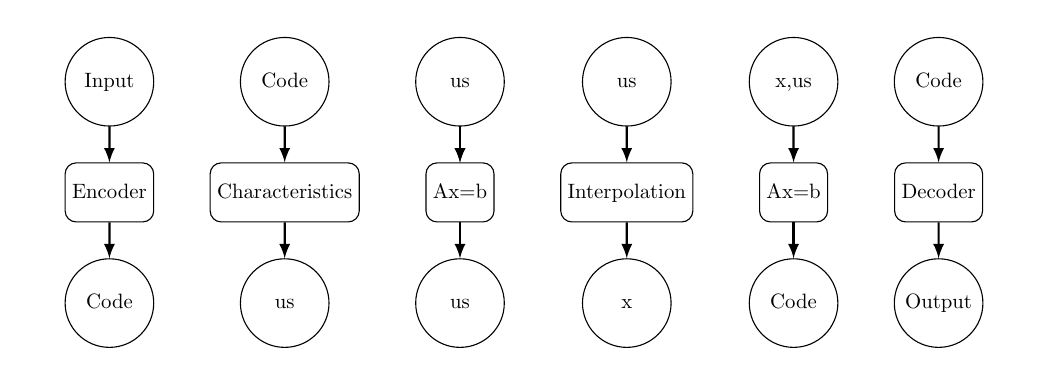
\begin{tikzpicture}[>=latex,text height=1.5ex,text depth=0.25ex,scale=.5,every node/.style={scale=0.75}]
		\matrix[matrix of nodes,column sep= 1em,row sep= 3ex]{
			&
			\node[circ] (1) {Input};&
			&
			\node[circ] (4) {Code};&
			&
			\node[circ] (7) {us};&
			&
			\node[circ] (10) {us};&
			&
			\node[circ] (13) {x,us};&
			&
			\node[circ] (16) {Code};&
			\\
			&
			\node[rec] (2) {Encoder};&
			&
			\node[rec] (5) {Characteristics};&
			&
			\node[rec] (8) {Ax=b};&
			&
			\node[rec] (11) {Interpolation};&
			&
			\node[rec] (14) {Ax=b};&
			&
			\node[rec] (17) {Decoder};&
			\\
			&
			\node[circ] (3) {Code};&
			&
			\node[circ] (6) {us};&
			&
			\node[circ] (9) {us};&
			&
			\node[circ] (12) {x};&
			&
			\node[circ] (15) {Code};&
			&
			\node[circ] (18) {Output};&
			\\
		};
	\path[->]
		(1) edge[thick] (2)
		(2) edge[thick] (3)
		(4) edge[thick] (5)
		(5) edge[thick] (6)
		(7) edge[thick] (8)
		(7) edge[thick] (8)
		(8) edge[thick] (9)
		(10) edge[thick] (11)
		(11) edge[thick] (12)
		(13) edge[thick] (14)
		(14) edge[thick] (15)
		(16) edge[thick] (17)
		(17) edge[thick] (18);
\end{tikzpicture}
	\caption{This figure shows the steps for obtaining a reduced oder model (ROM). Decoder and Encoder need to be used after training. In step one $y_0$ is the original input data, $C$ is the Code. In step two $c_i$ is the i-th intrinsic variable and $u_i$ the correspnding characteristic. The eigenvalue problem in step 3 outputs $x_i$ the eigenvector of A, a diagonal matrix composed of $u_i$ and b is the corresponing i-th intrinsic variable $c_i$. In step 4 $\hat{u}_i$ is the interpolated vector to $u_i$. Step 5 solves the linear equation for the diagonal matrix A composed of $\hat{u}_i$ times the eigenvector $x_i$ of the eigenvalueproblem in step 3. The output is $\hat{c}_i$ the i-th intrinsic variable corresponding to $\hat{u}_i$ the i-th interpolated characteristic.}
	\label{Fig. Flowchart}
\end{figure}